% main.tex, to be used with thesis.tex
% This contains the main work of your thesis.

%\bibliography{thesis}  % uses the references stored in Chapter1Radar.bib

\chapter{Conclusions and Future Works}

There were significant trends covered in this work, including the importance
that sensor networks are becoming ubiquitous, having their produced data
available online and other types of media. In the scope of Environmental Sensor
Networks, the collected data is the most important parameter to real-world
applications based on sensor networks. For example, the data collected in the
water may determine if a river is polluted, while the data collected during a
heavy snowfall can indicate hazard alerts the population. However, in order to
provide access to the collected data, one must first assess the different types of
infrastructural characteristics of the studied sensor networks. The selection
of a technology that provides such a persistence solution capabilities can be
part of a process of analysis of taxonomies proposed by this work,
characterized as the first contribution of this report.

Based on the findings of the taxonomies, together with the empirical analysis
of the technologies, this work revealed a novel approach to provide
persistence and access to collected data from sensor devices using the
Key-Value-Pair data model. Besides the contribution of a new component for the
Data Sensor Platform, the evidence that the system improves productivity was
confirmed during the execution of the experiments, writing less source-code to
obtain better functionalities when compared to other solutions. Similarly,
this work suggests that the abstraction of programming language should be
used with research groups whose primary expertise is not in Computer Science
or Database Systems.

The DSP Data Persistence component improves NetBEAMS's support to SF-BEAMS,
incorporating a persistence layer for the sensor network that can be used in
different ways. The solution for data persistence using Key-Value Pair
databases is a novel way to save collected data from sensor devices into a
single or multiple servers of a database technology. mongoDB's ability to cope
with the uncertainty of any properties collected from any sensor specification
is the most compelling reason to use the Key-value pair data model for collected
data from sensor devices.

As far as future works, there are many different directions for exploration.
The first major release of mongoDB with complete support to shards is
scheduled for 2010. An important mechanism of mongoDB is that it can
manage different mongoDB servers spread out in a cluster. This feature will give
better support to the Data-Centric Storage approach. This approach can reduce
the retrieval time by focusing on centralized selection of data over a given
database shard. Moreover, the overall search through the collected data
attributes can be drastically decreased by a parallel search over the database
shards using the MapReduce \cite{map-reduce} tools. At the time of development
of the experiments, the MapReduce API from mongoDB was also in the alpha
version, and therefore, presented many bugs. One suggestion for the
implementation of such functionality is based in Figure
\ref{fig:future-works-data-centric-map-reduce} (\cite{map-reduce-notes}), which
shows an architectural idea of the deployment of a Data-Centric storage approach. One scenario of
data retrieval is when a given processing in the search results are
required to be executed in parallel. The task of querying broken down into
two phases: the definition of the reduced problem as the parts, and the
mapping of the final result calculated with the response from each part. If
``Task" is considered to be a query (arrow 1) tor the server, then the
execution of the same query occurs in all different partitions (arrow 2), or
mongoDB shards. After processing the request, each node returns the result of
the query to the server (arrow 3), whose responsibility is to process each
individual result and return the final Result to the client application (arrow
4).

\begin{figure}[!h]
  \centering
  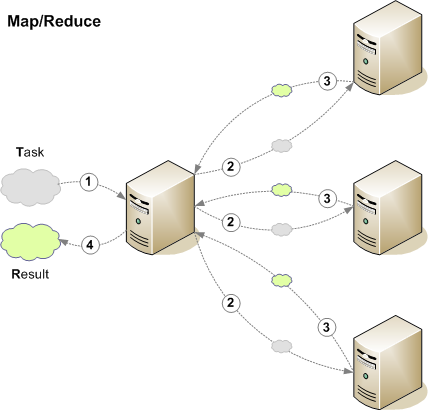
\includegraphics[scale=0.65]{../diagrams/future-works-data-centric-map-reduce}
  \caption{Data-Centric approach using MapReduce (\cite{map-reduce-notes})}
  \label{fig:future-works-data-centric-map-reduce}
\end{figure}

In addition to the infrastructure, the use  scheduling techniques for
data gathering in sensor networks can help the SF-BEAMS sensor networks
decrease the data load into the system. While the period of times used by RTC
seems to cover the basic requirements of data, the data storage may be seen as
overloaded with repeated data. Since environmental conditions might not change
drastically over time, the use of data scheduling and data clustering
approaches can be used. Considering that SF-BEAMS contains a cluster of
sensors, the data load could be decreased by using techniques such as
clustering the data in the data sink before they are persisted
\cite{sn-time-series, sn-schedule-minimal-aggregation-time}. Since the
infrastructure of the SF-BEAMS sensor network is a one-hop start design, the
knowledge about the data can only be achieved in the data sink. One suggestion
is the implementation of a DSP Data Clustering component that is responsible
for the data clustering before they are inserted into the database. Similarly,
the use of schedulers on the sensors could also be used to decrease the amount
of data to be sent to the data sink, as seen at the survey
\cite{sn-scheduling-survey}.

Finally, taking into account the use of the database system to complement
NetBEAMS execution, the design of event-based applications could add different
functionalities to the management capabilities of the sensor networks. For
instance, the collected data from a YSI device \cite{YSI-Sonde} carries the
information regarding the battery life of the device, seen at the collected
attribute ``observation.Battery''. A new DSP Component responsible for
observing these attributes could define the threshold of the event of
low-battery. With an event-based application in mind, events regarding the
SF-BEAMS network could be better managed through NetBEAMS where scheduled
sites visits would depend on such events to happen and, thus, avoiding
unnecessary operational costs.
